% Laborationsmall.tex
\documentclass[a4paper]{article}

\usepackage[swedish]{babel}
\usepackage[utf8x]{inputenc}

\usepackage{multicol}
\usepackage[vmargin=3cm,hmargin=2cm]{geometry}
\usepackage{parskip}
\usepackage[runin]{abstract}
\renewcommand{\abstitleskip}{0mm}

\usepackage{hyperref}
\usepackage{amsmath}
\usepackage{amsfonts}
\usepackage{lmodern}
\usepackage[T1]{fontenc}
\usepackage{pgfplots}
\pgfplotsset{compat=1.13}
\usetikzlibrary{decorations.pathreplacing}
\usetikzlibrary{arrows.meta}
\usepackage{pgfplotstable}
\usepackage{placeins}
\usepackage{siunitx}
\usepackage[numbered,framed]{matlab-prettifier}

\lstset{
	style              = Matlab-editor,
	basicstyle         = \mlttfamily,
	mlshowsectionrules = true,
}

\addto\extrasswedish{%
	\def\equationautorefname{Ekvation}%
	\def\figureautorefname{Figur}%
	\def\tableautorefname{Tabell}%
	\def\sectionautorefname{Rubrik}%
	\def\subsectionautorefname{Underrubrik}%
	\def\pageautorefname{Sida}%
}

\usepackage{graphicx}
%\usepackage{subcaption}
\usepackage{ccaption}
\captionnamefont{\it}
\captiontitlefont{\it}

% Hack för att få komma istället för punkt i matematiska uttryck
% $3.141592$ blir 3,141592
% Om man använder komma direkt får man ett litet oönskat mellanrum:
% $3,141592$ blir 3, 141592
\DeclareMathSymbol{,}{\mathpunct}{letters}{"3B}
\DeclareMathSymbol{.}{\mathord}{letters}{"3B}
\DeclareMathSymbol{\decimal}{\mathord}{letters}{"3A}

% Kommando för att få icke-kursiva enheter i matematiska uttryck
% $10\unit{km}$ blir 10 km
\newcommand{\unit}[1]{\ensuremath{\,\mathrm{#1}}}

\usepackage{lastpage}
\usepackage{fancyhdr}
\pagestyle{fancy}
\fancyhf[C]{\thepage}
\fancyhead[C]{Våglära och optik, FAFF30}
\fancyhead[R,L]{}
\fancypagestyle{plain}{
  \fancyhead{}
}
%\setcounter{secnumdepth}{-1} % Stänger av numrering.

\title{Laborationen ”Polarisation”}
\author{Johan Boström\\Anton Johansson\\Lunds Universitet}

\makeatletter
%\renewcommand{\section}{\@startsection
%{section}%                   % the name
%{1}%                         % the level
%{0mm}%                       % the indent
%{-\baselineskip}%            % the before skip
%{0.5mm}%          % the after skip
%{\normalfont\bfseries}} % the style
%\renewcommand{\sectionmark}[1]{ }
%\renewcommand{\thesection}{}

\renewcommand*\maketitle{
  {
    \begin{center}
      {\huge\bfseries \@title}\\
      \vspace{5mm}
      {\large \@author}
    \end{center}
    \vspace{2mm}
  }
}
\makeatother

\begin{document}
\maketitle

\renewcommand{\abstractname}{Abstract} % Om vi vill ha titeln till abstracten på engelska.

%\begin{abstract}
  %Kort beskrivning  av resultaten (5-10  rader). Det ska inte  vara en innehållsbeskrivning (först gör vi det, sen använder vi den metoden, och så jämför vi det med de där tidigare kända resultaten, etc) utan vara   koncentrerat  till   ”resultatet”,   vad   man  kommer fram till. Sammanfattningen är uppsatsens löpsedel. Den ska vara kort och kärnfull och locka läsare genom att  effektivt göra klart vad det är man uppnår genom att läsa rapporten.
  
%\end{abstract}

\vspace{2mm}

\hspace{-3mm}
\begin{tabular}{ll}
Laborationen genomförd: &	2017-05-09 \\
%Rapporten kamratgranskad: &	2013-xx-xx \\
Lämnad till handledare: &	2017-05-16 \\
\end{tabular}

\vspace{3mm}

\section{Inledning}
  %Preliminär beskrivning av uppgiften  i lättfattliga termer. Bakgrunden till att man intresserar sig för detta problem, denna uppgift. Hur den ingår i ett större sammanhang.

%  En detaljerad beskrivning av vad det hela går ut på, och vad exakt din uppgift   i    sammanhanget   är.    Utrustningsförutsättningar.   Det
%  ursprungligen avsedda målet. Även den i ämnet oinsatte ska ha en ärlig
%  chans att förstå de stora dragen.
%
%  Beskrivning av hur rapporten är uppbyggd, för att göra det möjligt för
%  läsaren att förstå vad som  pågår, ge läsaren rätta förväntningar, och
%  för  att  underlätta direktåtkomst  av  för  den individuelle  läsaren
%  särskilt intressanta delar.

\section{Teori}

I en elektromagnetisk våg oscillerar det elektriska och magnetiska fältet i planet vinkelrätt mot utbredningsriktningen. Då det elektriska fältet är så mycket större än det magnetiska brukar ljusets polarisation definieras som det elektriska fältets riktning. I opolariserat ljus oscillerar det elektriska fältet i slumpmässiga riktningar. \cite[pp.~146--148]{pearsonIntroOpt}

För att beskriva en vågs polarisering inför man en bas $(\vec e_x, \vec e_y)$ i planet vinkelrätt mot utbredningsriktningen och uttrycker det elektriska fältet som \cite{labManual}

\begin{equation}
	\vec E = E_x \sin\left(k z - \omega t + \delta\right) \vec e_x + E_y \sin\left(k z - \omega t\right) \vec e_y
\end{equation}

där $k$ är vågtalet, $\omega$ är vinkelfrekvensen, $\delta$ är en konstant fasförskjutning och $E_x$ och $E_y$ är amplituderna i respektive riktningar. Ett viktigt specialfall är då $\delta = n\pi \,\, \left(n \in \mathbb{Z}\right)$ eller antingen $E_x=0$ eller $E_y=0$, i detta fall oscillerar fältet längs en linje och kallas planpolariserat. Om istället $E_x=E_y$ och $\delta = \left(2 n + 1\right)\frac{\pi}{2}$ har det elektriska fältet alltid samma intensitet, men roterar i planet och kallas därför cirkulärpolariserat. \cite{labManual}\cite[p.~147]{pearsonIntroOpt}

Vissa material, till exempel kvarts, har egenskapen att brytningsindex skiljer sig mellan olika polarisationer. Kvarts är ett så kallat uniaxialt material, vilka har samma brytningsindex i två riktningar, men ett annat brytningsindex i den tredje riktningen. Riktningen med annorlunda brytningsindex brukar kallas för den optiska axeln. Detta innebär att polarisationer parallella med den optiska axeln kommer att röra sig med en annan hastighet än de som är vinkelräta.\cite{labManual}\cite[pp.~382--383]{pearsonIntroOpt}

I resten av rapporten kommer infallande ljus antas vara linjärpolariserat.

\subsection{Rörelse vinkelrätt mot den optiska axeln}

Om polarisationen av det infallande ljuset varken är vinkelrät mot eller parallell med den optiska axeln kan man dela upp den i två nollskilda vågor polariserade parallellt med respektive vinkelrätt mot den optiska axeln. Dessa delvågor kommer då ha olika brytningsindex och därmed ha olika fas då de lämnar materialet igen enligt \cite{labManual}

\begin{equation}
	\delta = \frac{2\pi}{\lambda} d \Delta n
	\label{eq:phaseDiff}
\end{equation}

där $\delta$ är fasförskjutningen, $\lambda$ är våglängden, $d$ är materialets tjocklek och $\Delta n$ är skillnaden i brytningsindex mellan de två polarisationerna.

I en experimentuppställning med en kristall utföljd av en analysator vinklad vinkelrätt mot det infallande ljusets polarisation kommer intensiteten $I$ beräknas med \cite{labManual}

\begin{equation}
	I = I_0 \sin\left(2\theta\right)^2 \sin\left(\delta / 2\right)^2
\end{equation}

där $\theta$ är vinkeln mellan det infallande ljusets polarisation och den optiska axeln. Maximal intensitet uppkommer då när $\sin\left(\delta / 2\right) = \pm 1$, eller $\delta = \left(2 n + 1\right)\pi$. \cite{labManual} Med detta tillsammans med \eqref{eq:phaseDiff} är alltså villkoret för maxima

\begin{equation}
	d \Delta n = \left(2 (m - p) + 1\right)\frac{\lambda}{2}\text{.}
	\label{eq:deltaMax}
\end{equation}

där $p$ är ett heltal som bestämmer ordningen relativt ett fast maximum $m$ och som ökar med ökande våglängd då $d \Delta n$ är ungefär konstant mellan två närliggande maxima.

För att beräkna brytningsindexets beroende av våglängden kan den empiriskt framtagna Cauchys formel användas \cite{labManual} \cite[p.~67]{pearsonIntroOpt}

\begin{equation}
	n = a + \frac{b}{\lambda^2}
\end{equation}

där $a$ och $b$ är konstanter. Då differansen av två ekvationer på denna form har exakt samma form kan även skillnaden i brytningsindex skrivas

\begin{equation}
	\Delta n = A + \frac{B}{\lambda^2}
	\label{eq:deltaCauchy}
\end{equation}

med två nya konstanter $A$ och $B$. Detta kan kombineras med \eqref{eq:phaseDiff} till

\begin{equation}
	d \left(A + \frac{B}{\lambda^2}\right) = \left(2 (m - p) + 1\right)\frac{\lambda}{2}\text{.}
	\label{eq:cauchyMax}
\end{equation}

Om man våglängderna av ett antal maxima mitt i ett spektrum kan man då använda denna formel för att anpassa en kurva med de tre konstanterna $A$, $B$ och $m$.

\subsection{Rörelse parallellt med den optiska axeln}

Då den infallande ljusstrålen instället rör sig parallellt med den optiska axeln kommer polarisationen alltid att vara vinkelrätt mot den optiska axeln och påverkas därför inte av att kristallen har ett annorlunda brytningsindex. Svagare effekter av kristallstrukturen går då att se, varav en viktig effekt kallas optisk aktivitet och innebär att polarisationsplanet roteras. Matematiskt kan detta beskrivas genom att cirkulärpolariserade vågor som roterar åt olika håll har olika brytningsindex. Då kommer den ena cirkulärpolariserade vågen ha fått ett fasskifte efter kristalllen och summan kommer att bli en likadan men roterad polarisation jämfört med den infallande polarisationen. \cite{labManual} \cite[pp.~387--391]{pearsonIntroOpt}

Med samma argument som för dubbelbrytning kan våglängdsberoendet beskrivas med \cite{labManual}

\begin{equation}
	\rho = a + \frac{b}{\lambda^2}
\end{equation}

där $\rho$ är rotationen per längdenhet. Här ser man att längre våglängder kommer roteras mindre än korta.

Beroende på om rotationen sker moturs eller medurs relativt en observatör som tittar mot ljuskällan kallas materialet för dextero- respektive levorotatory. Detta är oberoende av vilket håll som ljuset infaller från, vilket kan inses genom att gå igenom processen baklänges.

\subsection{Polarisation och reflektans}



\section{Metod}
  % De  olika  stegen  i  uppgiftens genomförande.  Till  exempel  val  av
  % algoritmer,  programspråk och  annan programvara,  undersökningsmetod,
  % statistiska  metoder. Där  valmöjligheter finns,  diskutera de  gjorda
  % valen.
  
  I alla experiment användes en vitljuslampa vars ljus linjerades genom en polarisator och en analysator in i en kalibrerad spektrometer som mätte intensiteten av ljus i våglängdsintervallet mellan cirka \SI{480}{\nano\meter} till \SI{720}{\nano\meter} med en CCD inkopplad till en dator.
  
  I första experimentet placerades tre kvartskristaller en åt gången mellan polarisatorn och analysatorn. Kristallerna var klyvda längs den optiska axeln med tjocklekarna \SI{0.24}{\milli\meter}, \SI{1}{\milli\meter} respektive \SI{3}{\milli\meter}. Kristallerna roterades så att deras effekter på spektrumet blev så liten respektive stor som möjligt och därefter roterades analysatorn och det registrerade spektrumet sparades vid intressanta vinklar av analysatorn. På den tjockaste kristallen mätte vi även våglängderna för 11 toppar mellan cirka \SI{500}{\nano\meter} till \SI{600}{\nano\meter}.
  
  I andra experimentet placerades en tjockare kvartskristall med en tjocklek av storleksordningen centimetrar och klyvd mot den optiska axeln mellan polarisatorn och analysatorn. Spektrumets observerades då analysatorn roterades och några bilder togs.
  
  Till sist togs analysatorn och alla kristaller bort och i ljusstrålens väg placerades istället en glasskiva. Polarisatorn och glasskivan roterade tills reflektionen på glasskivan försvann och vinkeln noterades.

\section{Resultat}

\FloatBarrier

\pgfmathsetmacro{\A}{0.009081}
\pgfmathsetmacro{\B}{0.0001519}
\pgfmathsetmacro{\m}{58}
%\pgfmathsetmacro{\A}{0.009356}
%\pgfmathsetmacro{\B}{0.0001245}
%\pgfmathsetmacro{\m}{59}
\pgfmathsetmacro{\d}{3000}
\pgfmathsetmacro{\maxM}{\m-1}
\pgfmathsetmacro{\minM}{\m-11}

\begin{figure}[ht]
	\centering
	\begin{tikzpicture}
	\begin{axis}[
	title=Skillnad i brytningsindex som funktion av våglängd,
	grid=both,
	xlabel=$\lambda$/\si{\micro\meter},
	ylabel=$\Delta n$,
	xmin=0.45,
	xmax=0.75,
	scaled ticks=false,
	y tick label style={/pgf/number format/.cd,sci,sci e}
	]
	\addplot[mark=none,blue,domain=0.45:0.75] {\A + \B/x^2};
	\addlegendentry{anpassad kurva};
	\addplot[only marks,mark=+,red] coordinates {
		(0.504870000000000, 0.009676675000000)
		(0.512890000000000, 0.009659428333333)
		(0.521150000000000, 0.009641275000000)
		(0.529640000000000, 0.009621793333333)
		(0.538600000000000, 0.009605033333333)
		(0.547800000000000, 0.009586500000000)
		(0.557470000000000, 0.009569901666667)
		(0.567610000000000, 0.009554768333333)
		(0.577980000000000, 0.009536670000000)
		(0.588820000000000, 0.009519256666667)
		(0.600120000000000, 0.009501900000000)
	};
	\addlegendentry{datapunkter};
	\end{axis}
	\end{tikzpicture}
	\caption{Skillnad i brytningsindex beräknade med \eqref{eq:deltaMax} från datan samt funktionen \eqref{eq:deltaCauchy}. $A$, $B$ och $m$ togs fram genom en anpassning av \eqref{eq:cauchyMax} där $A$, $B$ och $m$ tilläts variera. Bästa anpassning gav $A=\SI{\A}{}$, $B=\SI{\B}{\micro\meter\squared}$ och $m=\m$.}
\end{figure}

\FloatBarrier

medurs från observatör
+ = 180 -> 360
- = 180 -> 0

\FloatBarrier
\begin{figure}[h!]
	\centering
	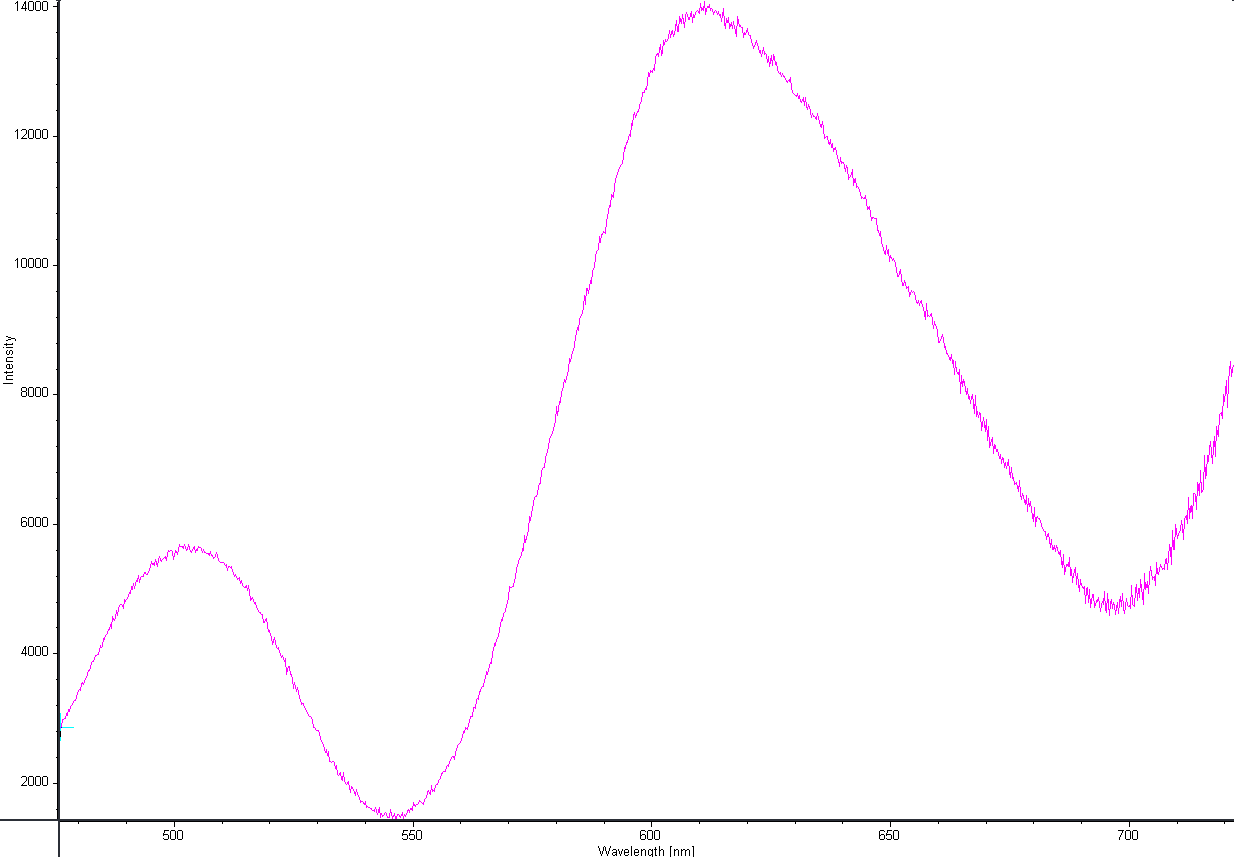
\includegraphics[width=\linewidth]{data/spektra_180_kristall1_180_inv}
	\caption{Intensitetsspektra för en \SI{0.24}{\milli\m} tjock kvartskristall, där ljuset infaller vinkelrätt mot den optiska axeln. Polarisatorn och analysatorn är båda vertikala med en vinkel på \SI{180}{\degree}.}
	\label{fig:}
\end{figure}
\FloatBarrier

\FloatBarrier
\begin{figure}[h!]
	\centering
	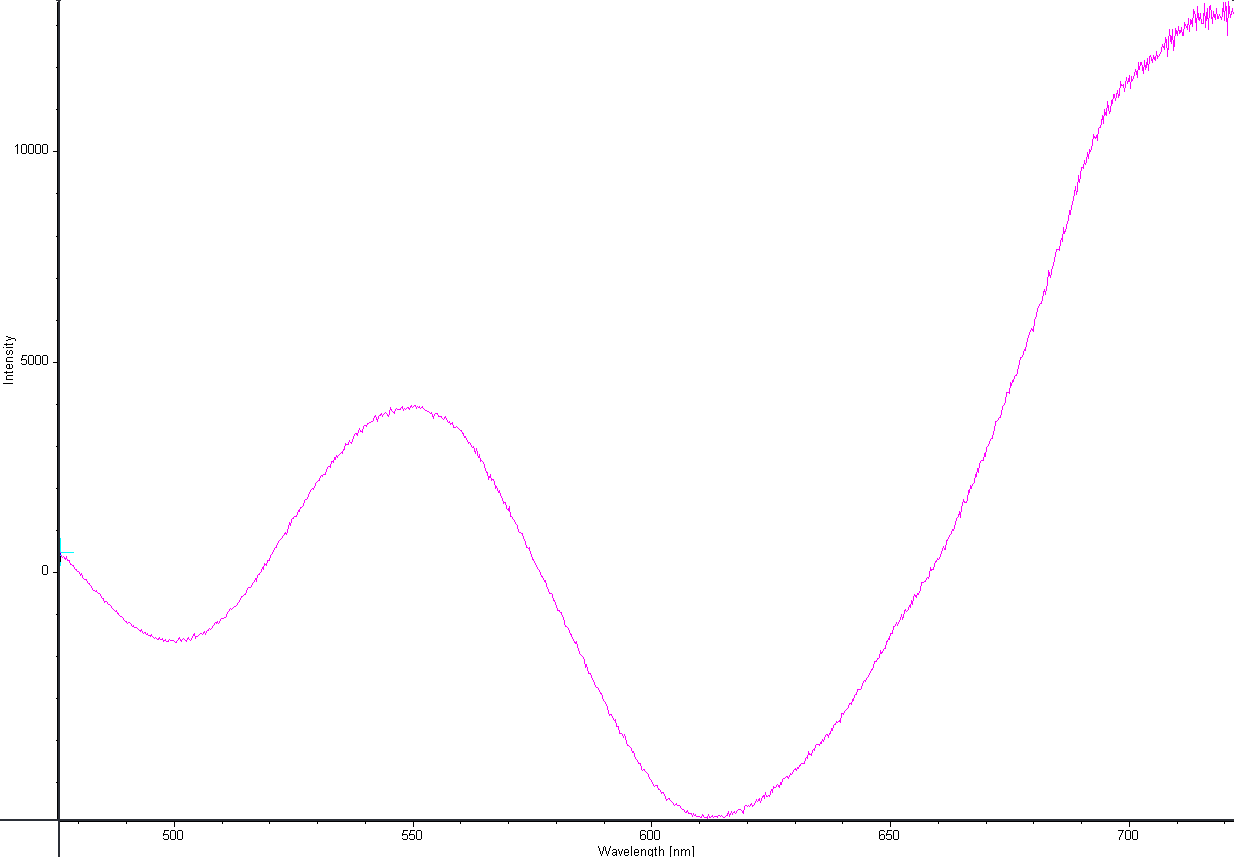
\includegraphics[width=\linewidth]{data/spektra_180_kristall1_270_inv}
	\caption{Intensitetsspektra för en \SI{0.24}{\milli\m} tjock kvartskristall, där ljuset infaller vinkelrätt mot den optiska axeln. Analysatorn är vinkelrät med hänsyn på Polarisatorn.}
	\label{fig:}
\end{figure}
\FloatBarrier

\FloatBarrier
\begin{figure}[h!]
	\centering
	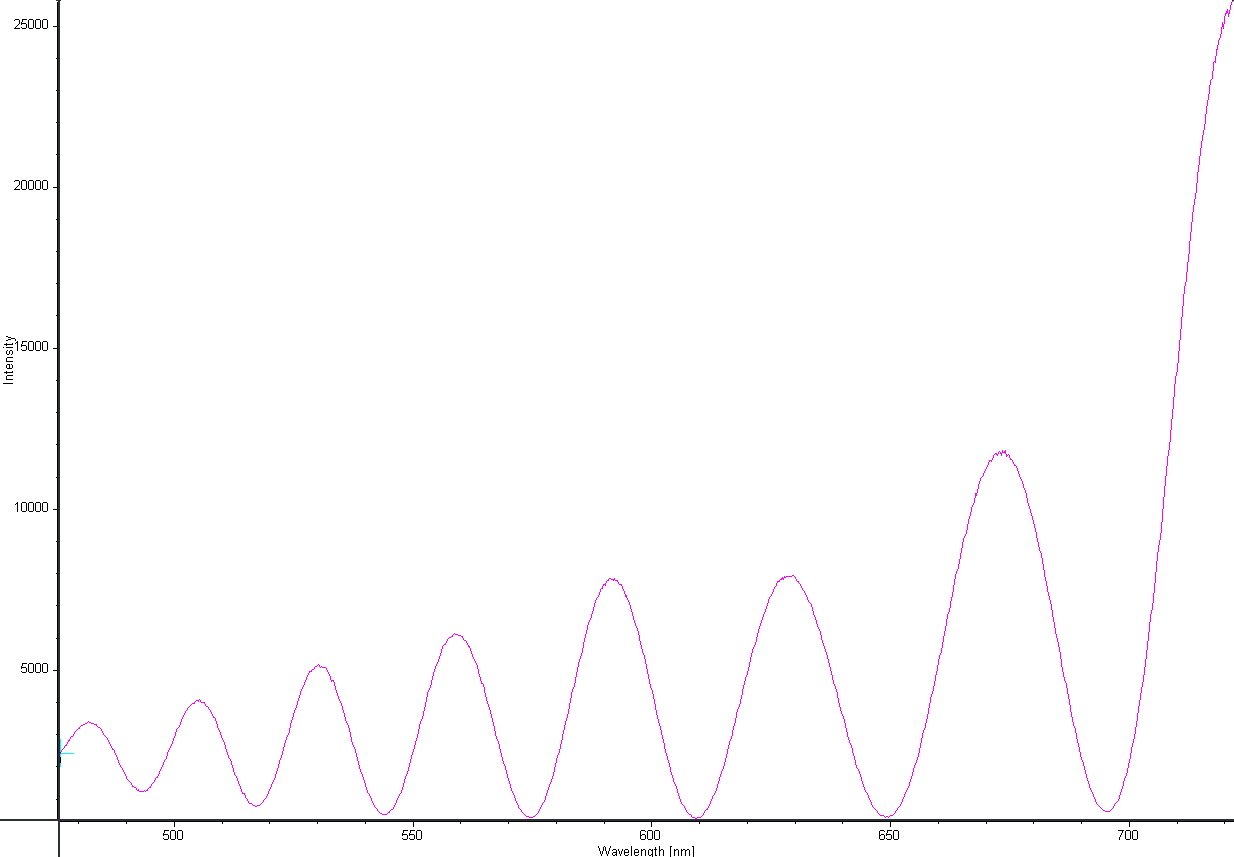
\includegraphics[width=\linewidth]{data/spektra_180_kristall2_0_inv}
	\caption{Intensitetsspektra för en \SI{1}{\milli\m} tjock kvartskristall, där ljuset infaller vinkelrätt mot den optiska axeln.  Polarisatorn och analysatorn är båda vertikala med en vinkel på \SI{180}{\degree}}
	\label{fig:}
\end{figure}
\FloatBarrier	

\FloatBarrier
\begin{figure}[h!]
	\centering
	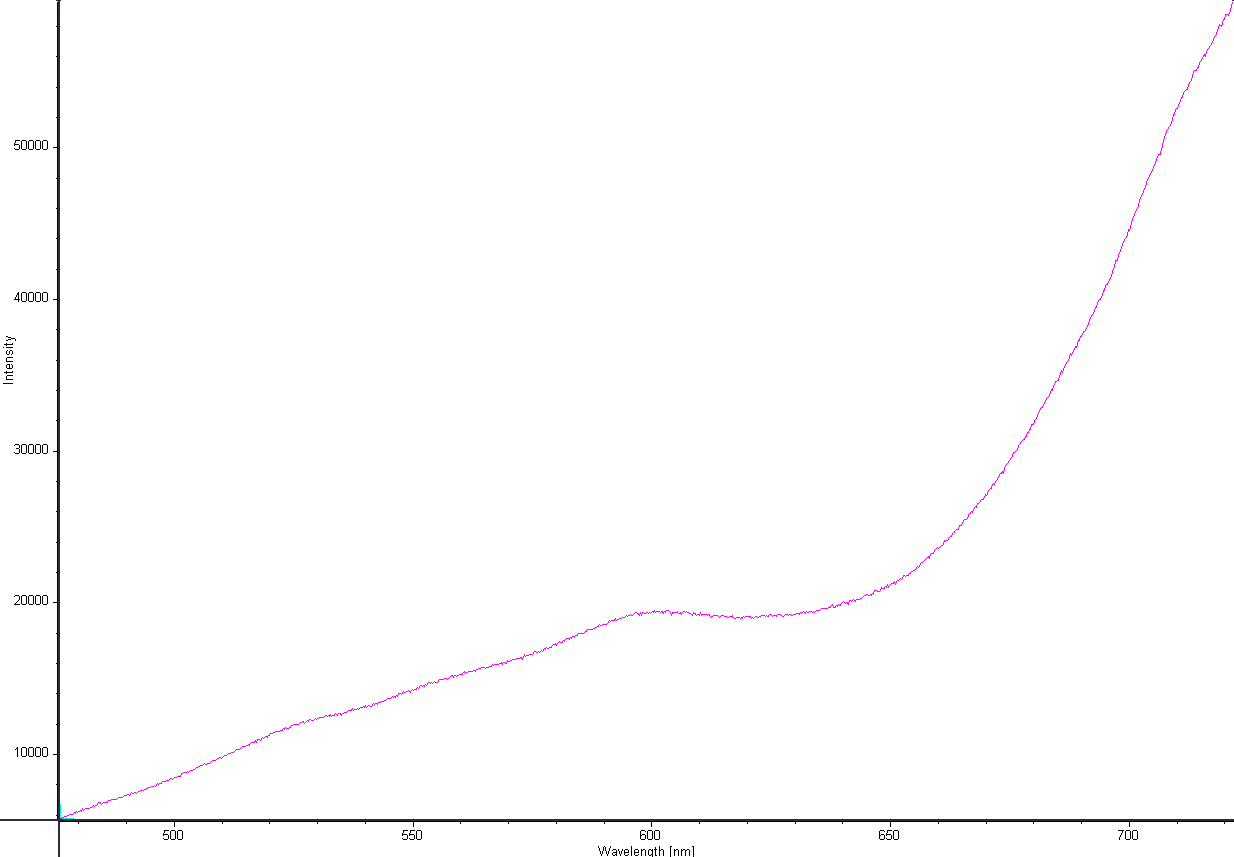
\includegraphics[width=\linewidth]{data/spektra_180_kristall2_70_inv}
	\caption{...}
	\label{fig:}
\end{figure}
\FloatBarrier

\FloatBarrier
\begin{figure}[h!]
	\centering
	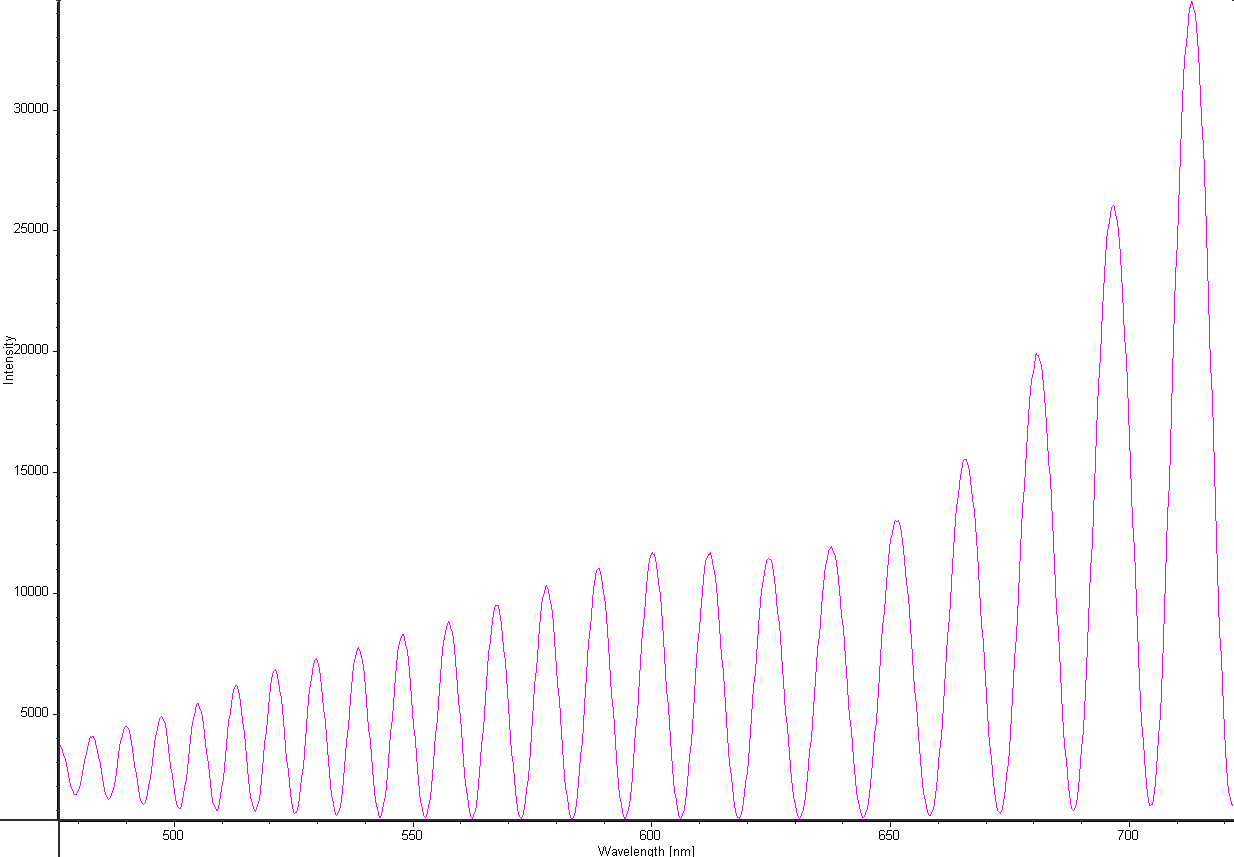
\includegraphics[width=\linewidth]{data/spektra_180_kristall3_140_inv}
	\caption{...}
	\label{fig:}
\end{figure}
\FloatBarrier

\FloatBarrier
\begin{figure}[h!]
	\centering
	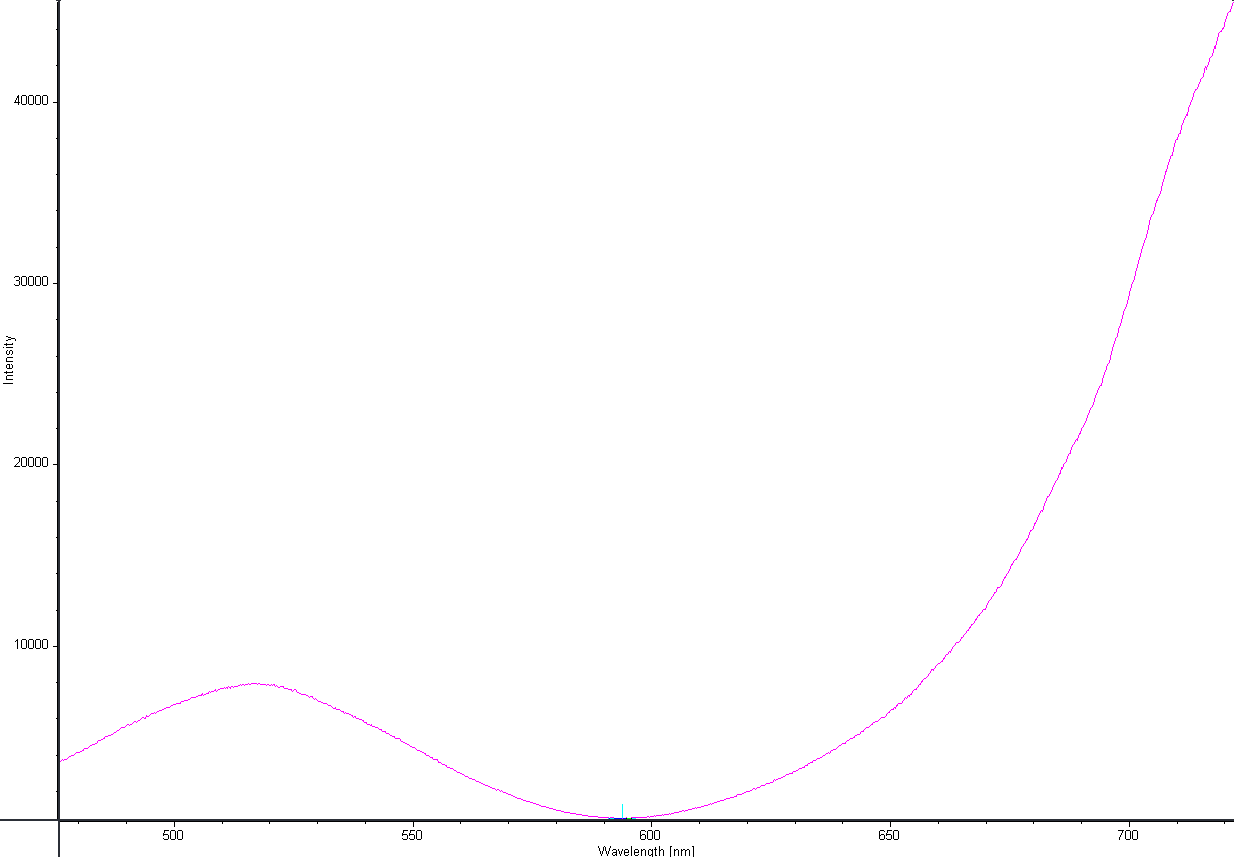
\includegraphics[width=\linewidth]{data/spektra_aktiv1_inv}
	\caption{...}
	\label{fig:}
\end{figure}
\FloatBarrier

\FloatBarrier
\begin{figure}[h!]
	\centering
	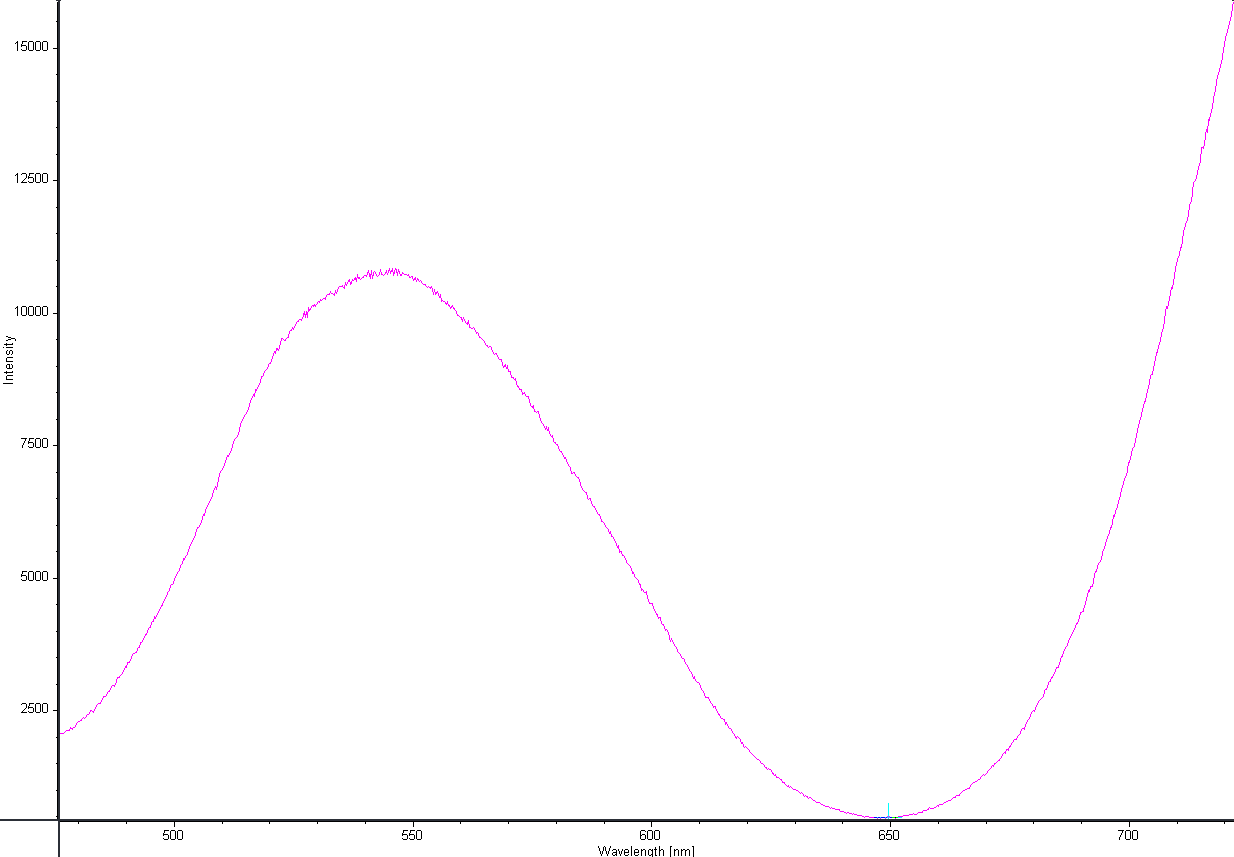
\includegraphics[width=\linewidth]{data/spektra_aktiv2_inv}
	\caption{...}
	\label{fig:}
\end{figure}
\FloatBarrier

\FloatBarrier
\begin{figure}[h!]
	\centering
	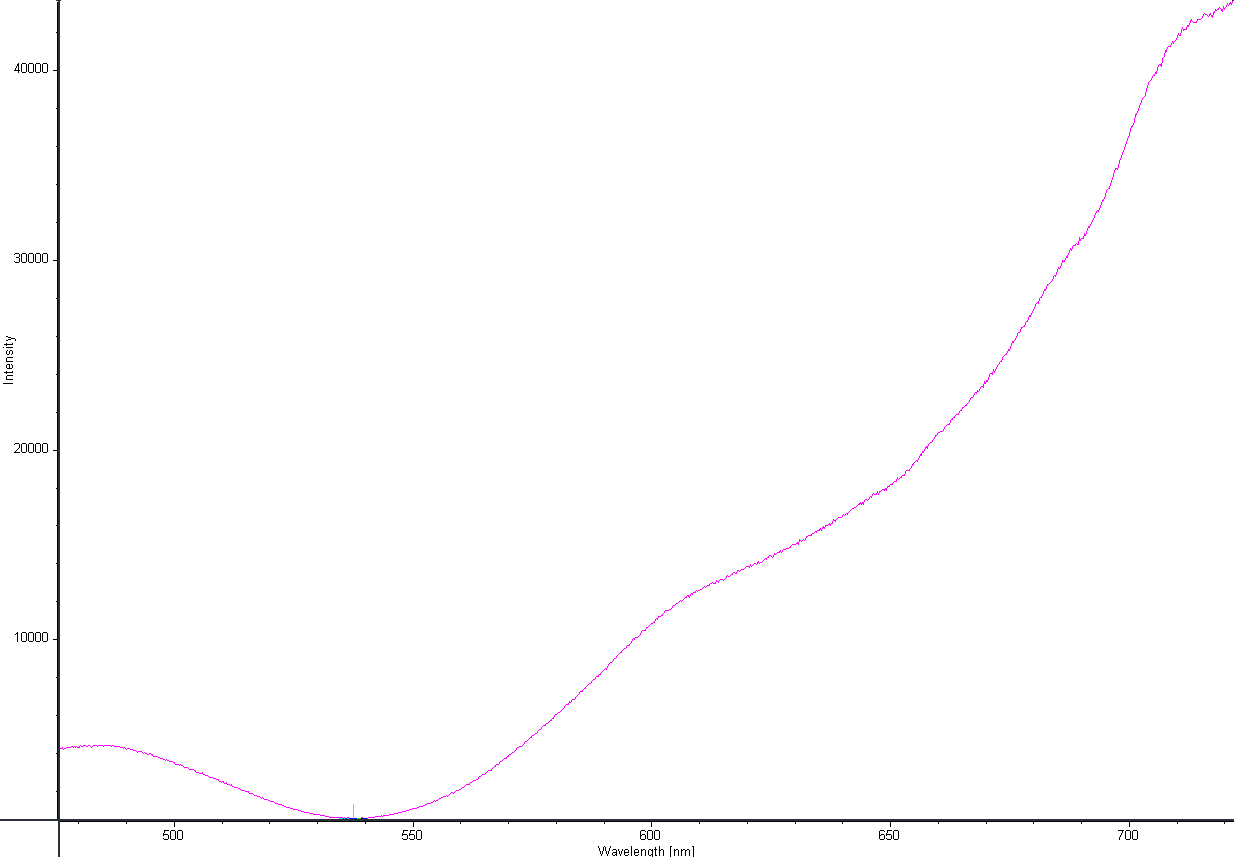
\includegraphics[width=\linewidth]{data/spektra_aktiv3_inv}
	\caption{...}
	\label{fig:}
\end{figure}
\FloatBarrier

\FloatBarrier
\begin{figure}[h!]
	\centering
	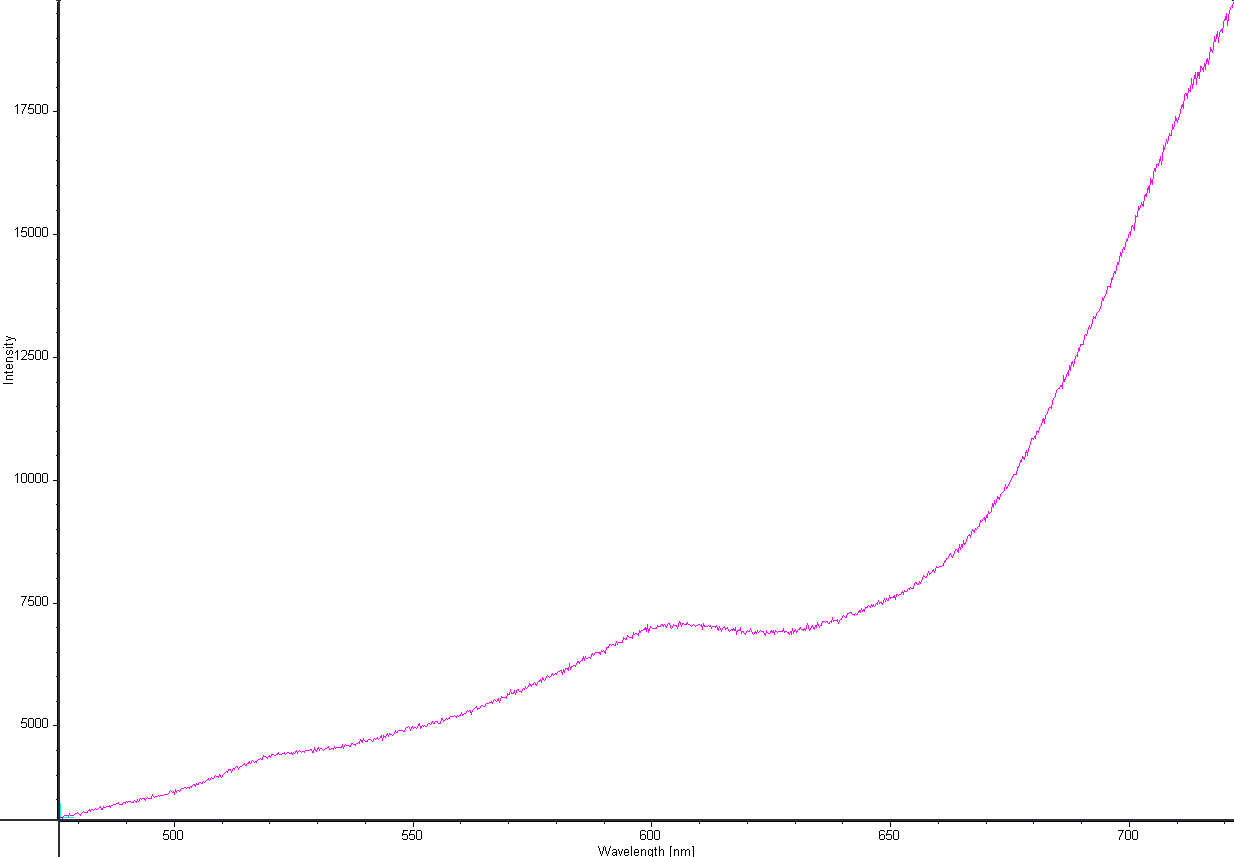
\includegraphics[width=\linewidth]{data/spektra_kristall1_optAx_inv}
	\caption{...}
	\label{fig:}
\end{figure}
\FloatBarrier

\section{Diskussion}
  %Är resultaten rimliga? Vad hade kunnat göras annorlunda?

%\section{Slutsats}
  %En   sammanfattning  där   man  till   skillnad  från   den  inledande
  %sammanfattningen förutsätter  att läsaren har läst  rapporten, samt de
  %slutsatser man kan dra av det gjorda arbetet.
 
 \bibliography{bibliography}{}
 \bibliographystyle{plain}

\end{document}
